\section{Heur\'istica Golosa}
\subsection{Explicacion detallada de la heur\'istica propuesta}

La heur\'istica desarrollada consiste en una modificaci\'on del algoritmo de camino m\'inimo de Dijkstra.

\subsubsection{Inicializaci\'on}

En la etapa de inicializaci\'on se declaran cuatro vectores a utilizar:

\begin{enumerate}

\item CostosW2
\item Predecesores
\item CostoCamino
\item CostosW1
\end{enumerate}

CostosW2, es an\'alogo al vector distancias del algoritmo de Dijkstra, siendo $w_2$ la distancia a minimizar, guarda el costo del camino provisorio que va armando el algoritmo. Predecesores es an\'alogo al vector predecesores de dicho algoritmo, indicando para cada nodo cu\'al es su predecesor en dicho camino, mientras que CostoCamino almacena su costo $w_1$.

\vspace{2mm}

CostosW1 almacena el costo $w_1$ del camino m\'inimo de cada nodo hasta el nodo de llegada, por razones que explicamos a continuaci\'on:

\vspace{2mm}

Luego de la declaraci\'on de los vectores, se calculan los caminos m\'inimos en cuanto a costo $w_1$ de todos los nodos hacia el nodo de llegada. Ya que el grafo es simple, las aristas no tienen orientaci\'on definida, por lo cual dados dos nodos $v_1$ y $v_2$, el camino m\'inimo de $v_1$ a $v_2$ es igual al camino m\'inimo de $v_2$ a $v_1$. Esto nos permite ejecutar una \'unica vez el algoritmo de Dikjstra desde el nodo de llegada hasta todos los dem\'as sobre $w_1$ y obtener lo buscado.

\vspace{2mm}

Una vez obtenidos los caminos m\'inimos de cada nodo a la llegada en cuanto a costo $w_1$, \'estos nos permiten conocer lo siguiente:

\begin{enumerate}
\item Al iniciar el algoritmo, aquellos nodos para las cuales no existe un camino de longitud $w_1 \leq K$ hasta el nodo llegada, los cuales nuestro algoritmo va a ignorar.
\item En medio de la ejecuci\'on del algoritmo, desde un nodo $v$ podemos saber si el nodo $x$ de la pro\'oxima arista $(v,x$) a considerar tiene al menos un camino $c$ hasta el nodo llegada tal que, el costo del camino formado por la uni\'on de $c$ ($costoW1(x)$) y el recorrido hasta ahora ($costoCamino(v)$) es $\leq K$. En caso de no tenerlo, desde ese nodo no hay un camino v\'alido hasta la llegada, por lo tanto nuestro algoritmo va a descartar esta arista y elegir alguna que tenga al menos un camino posible hasta la llegada. Esto lo podemos conocer, ya que la ejecuci\'on de Dijkstra inicial nos brinda el costo $w_1$ del camino m\'inimo desde el nodo $x$ hasta la llegada, por lo tanto  si $costoCamino(v)$ + $costo(v,x)$ + $Costosw_1(x)$ $\leq$ $K$ sabemos que existe al menos este camino v\'alido, caso contrario descartamos la arista.
\end{enumerate}



\begin{center}
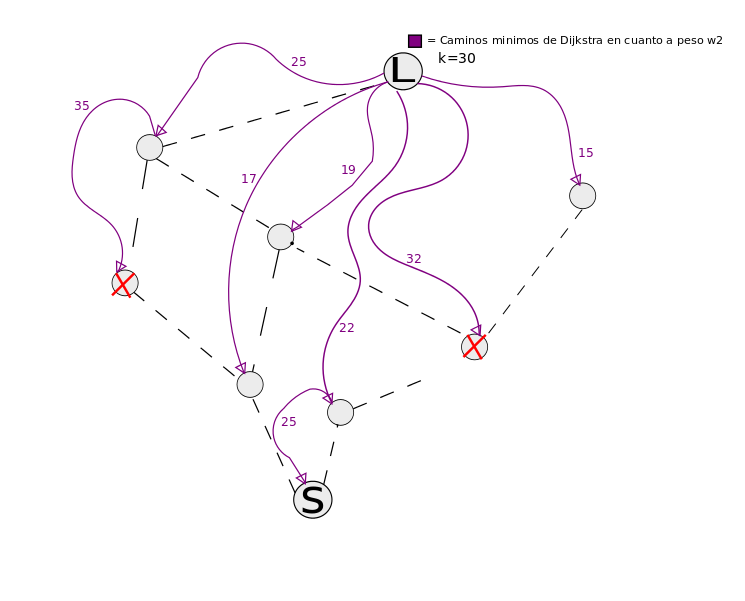
\includegraphics[scale=0.58]{img/inicializacion.png}
\end{center}	
\vspace{2mm}

Este dibujo representa la ejecuci\'on de la inicializaci\'on de la heur\'stica, donde el algoritmo de Dijkstra calcula los costos $w_1$ de los caminos m\'inimos de todos los nodos al nodo llegada (en violeta), y puede verse que aquellos nodos con caminos de costo mayor a $K$ ser\'an descartados.

\subsubsection{Heur\'istica golosa}

El algoritmo goloso en s\'i comparte su estructura con el algoritmo de Dijkstra, utilizando costos $w_2$. El agregado al algoritmo es la estrategia previamente explicada, teniendo la informaci\'on que nos brindan $CostosW1$ y $CostoCamino$, cuando sacamos un nodo $v$ de la cola y procedemos a actualizar sus vecinos $x$, s\'olo vamos a considerar actualizar los valores $CostosW2$ y $precedesor$ para aquellos que sean factibles, es decir, aquellos para los cuales el costo $w_1$ del camino m\'inimo $x$ - llegada + el costo de la arista entre los nodos $(v,x)$ + el costo $w_1$ del camino recorrido potencial recorrido hasta $v$ es menor o igual a K, dicho en t\'erminos del algoritmo: $CostosW1[x]+costo(v,x)+costoCamino[v]\leq K$. Esto nos asegura que el camino de un nodo nunca va a ser actualizado por un camino no factible.

\subsubsection{Pseudoc\'odigo}

\begin{algorithm}
	\caption{Heur\'istica Golosa}
\begin{algorithmic}[1]
\Statex

\Procedure{Heur\'istica Golosa}{grafo g, nodo u, nodo v, cota K}{ -$>$ camino}

\State $ vector<int> \: costosw_1[n] $
\Comment $O(n)$
\State $vector<int> costosw_2[n]$
\Comment $O(n)$
\State $vector<int> predecesores[n]$
\Comment $O(n)$
\State $ vector<int> \: costoCamino[n] $
\Comment $O(n)$
\State $camino \: c \gets [] $
\Comment $O(n^2)$
\State $colaPrioridad \: cola \gets []$
\Comment $O(1)$

\Statex

\State $ Dijkstra(g, v, costosw_1) $
\Comment $O(n^2)$

\Statex

\For{$i\: from \: 0 \: to \: n-1$}
\Comment $ O(n)$
	\State $ costosw_2[i] \gets \infty $
	\State $ predecesores[i] \gets NULL $
	\State $ costoCamino[i] \gets 0 $	
\EndFor

\State $ costosw_2[u] \gets 0 $
\Statex
\State $ cola.push(costosw_2, u) $

\While{$cola != []$}
	\Comment $ O(n)$
	\State $ par<costow_2, nodo> actual \gets cola.pop $
	\Comment $O(logn)$
	\For{$ w \: : \: adyacentes(actual_2) $}
		\Comment $ O(n)$
		\If{ $costoCamino[actual_2] + costosw_1(w) + costow_1Arista(actual_2,w) \leq K ORDENARR $ }
		

			\If{$ costosw_2[w] > costosw_2[actual_2] + costow_2Arista(actual,w) $}
			\Comment $O(logn)$
			\State $ costosw_2[w] \gets costosw_2[actual_2] + costow_2Arista(actual,w) $
			\State $ costoCamino[w] \gets costoCamino[actual_2] + costow_1Arista(actual_2,w) $
			\State $ predecesor[w] = actual $
			\State $cola.push(costow_2(w), w)$
			\Comment $O(logn)$


			\EndIf

		\EndIf
	\EndFor

\EndWhile

\State $ c \gets reconstruirCamino(predecesor,v) $
\State $ return \:c $

\EndProcedure
\end{algorithmic}
\end{algorithm}


s